%%%%%%%%%%%%%%%%%%%%%%%%%%%%%%%%%%%%%%%%%
% Nat64 support for IML
% Module cpib
%
% This template was downloaded from:
% http://www.LaTeXTemplates.com
%
% Authors:
% Marco Romanutti
% Benjamin Meyer
%
% License:
% CC BY-NC-SA 3.0 (http://creativecommons.org/licenses/by-nc-sa/3.0/)
%
%%%%%%%%%%%%%%%%%%%%%%%%%%%%%%%%%%%%%%%%%

%----------------------------------------------------------------------------------------
%	PACKAGES AND OTHER DOCUMENT CONFIGURATIONS
%----------------------------------------------------------------------------------------

\documentclass[10pt, a4paper, twocolumn]{article} % 10pt font size (11 and 12 also possible), A4 paper (letterpaper for US letter) and two column layout (remove for one column)

%%%%%%%%%%%%%%%%%%%%%%%%%%%%%%%%%%%%%%%%%
% Bloom filter
% Module dist
% Assignment 02
%
% This template was downloaded from:
% http://www.LaTeXTemplates.com
%
% Authors:
% Marco Romanutti
% Dominik Fringeli
%
% License:
% CC BY-NC-SA 3.0 (http://creativecommons.org/licenses/by-nc-sa/3.0/)
%
%%%%%%%%%%%%%%%%%%%%%%%%%%%%%%%%%%%%%%%%%

%----------------------------------------------------------------------------------------
%	PACKAGES AND OTHER DOCUMENT CONFIGURATIONS
%----------------------------------------------------------------------------------------

\usepackage[english]{babel} % English language hyphenation

\usepackage{microtype} % Better typography

\usepackage{amsmath,amsfonts,amsthm} % Math packages for equations

\usepackage[svgnames]{xcolor} % Enabling colors by their 'svgnames'

\usepackage[hang, small, labelfont=bf, up, textfont=it]{caption} % Custom captions under/above tables and figures

\usepackage{booktabs} % Horizontal rules in tables

\usepackage{lastpage} % Used to determine the number of pages in the document (for "Page X of Total")

\usepackage{graphicx} % Required for adding images
\usepackage{float} % Force image placement

\usepackage{enumitem} % Required for customising lists
\setlist{noitemsep} % Remove spacing between bullet/numbered list elements

\usepackage{sectsty} % Enables custom section titles

\usepackage{tabularx} % Pro/cons table
\allsectionsfont{\usefont{OT1}{phv}{b}{n}} % Change the font of all section commands (Helvetica)

\usepackage{ marvosym } % Symbols
%----------------------------------------------------------------------------------------
%	MARGINS AND SPACING
%----------------------------------------------------------------------------------------

\usepackage{geometry} % Required for adjusting page dimensions

\geometry{
	top=1cm, % Top margin
	bottom=1.5cm, % Bottom margin
	left=2cm, % Left margin
	right=2cm, % Right margin
	includehead, % Include space for a header
	includefoot, % Include space for a footer
	%showframe, % Uncomment to show how the type block is set on the page
}

\setlength{\columnsep}{7mm} % Column separation width

%----------------------------------------------------------------------------------------
%	FONTS
%----------------------------------------------------------------------------------------

\usepackage[T1]{fontenc} % Output font encoding for international characters
\usepackage[utf8]{inputenc} % Required for inputting international characters

\usepackage{XCharter} % Use the XCharter font

\usepackage{amssymb}% http://ctan.org/pkg/amssymb
\usepackage{pifont}% http://ctan.org/pkg/pifont
\newcommand{\cmark}{\ding{51}}%
\newcommand{\xmark}{\ding{55}}%

%----------------------------------------------------------------------------------------
%	HEADERS AND FOOTERS
%----------------------------------------------------------------------------------------

\usepackage{fancyhdr} % Needed to define custom headers/footers
\pagestyle{fancy} % Enables the custom headers/footers

\renewcommand{\headrulewidth}{0.0pt} % No header rule
\renewcommand{\footrulewidth}{0.4pt} % Thin footer rule

\renewcommand{\sectionmark}[1]{\markboth{#1}{}} % Removes the section number from the header when \leftmark is used

%\nouppercase\leftmark % Add this to one of the lines below if you want a section title in the header/footer

% Headers
\lhead{} % Left header
\chead{\textit{\thetitle}} % Center header - currently printing the article title
\rhead{} % Right header

% Footers
\lfoot{} % Left footer
\cfoot{} % Center footer
\rfoot{\footnotesize Seite \thepage\ von \pageref{LastPage}} % Right footer, "Page 1 of 2"

\fancypagestyle{firstpage}{ % Page style for the first page with the title
	\fancyhf{}
	\renewcommand{\footrulewidth}{0pt} % Suppress footer rule
}

%----------------------------------------------------------------------------------------
%	TITLE SECTION
%----------------------------------------------------------------------------------------

\newcommand{\authorstyle}[1]{{\large\usefont{OT1}{phv}{b}{n}\color{DarkRed}#1}} % Authors style (Helvetica)

\newcommand{\institution}[1]{{\footnotesize\usefont{OT1}{phv}{m}{sl}\color{Black}#1}} % Institutions style (Helvetica)

\usepackage{titling} % Allows custom title configuration

\newcommand{\HorRule}{\color{DarkGoldenrod}\rule{\linewidth}{1pt}} % Defines the gold horizontal rule around the title

\pretitle{
	\vspace{0pt} % Move the entire title section up
	\HorRule\vspace{10pt} % Horizontal rule before the title
	\fontsize{32}{36}\usefont{OT1}{phv}{b}{n}\selectfont % Helvetica
	\color{DarkRed} % Text colour for the title and author(s)
}

\posttitle{\par\vskip 15pt} % Whitespace under the title

\preauthor{} % Anything that will appear before \author is printed

\postauthor{ % Anything that will appear after \author is printed
	\vspace{10pt} % Space before the rule
	\par\HorRule % Horizontal rule after the title
	\vspace{-34pt} % Space after the title section
}

%----------------------------------------------------------------------------------------
%	ABSTRACT
%----------------------------------------------------------------------------------------

\usepackage{lettrine} % Package to accentuate the first letter of the text (lettrine)
\usepackage{fix-cm}	% Fixes the height of the lettrine

\newcommand{\initial}[1]{ % Defines the command and style for the lettrine
	\lettrine[lines=3,findent=4pt,nindent=0pt]{% Lettrine takes up 3 lines, the text to the right of it is indented 4pt and further indenting of lines 2+ is stopped
		\color{DarkGoldenrod}% Lettrine colour
		{#1}% The letter
	}{}%
}

\usepackage{xstring} % Required for string manipulation

\newcommand{\lettrineabstract}[1]{
	\StrLeft{#1}{1}[\firstletter] % Capture the first letter of the abstract for the lettrine
	\initial{\firstletter}\textbf{\StrGobbleLeft{#1}{1}} % Print the abstract with the first letter as a lettrine and the rest in bold
}

%----------------------------------------------------------------------------------------
%	LISTINGS
%----------------------------------------------------------------------------------------

\usepackage{listings}
\usepackage{color}
\usepackage[listings]{tcolorbox}

\definecolor{dkgreen}{rgb}{0,0.6,0}
\definecolor{gray}{rgb}{0.5,0.5,0.5}
\definecolor{mauve}{rgb}{0.58,0,0.82}

\lstset{frame=tb,
language=Java,
aboveskip=3mm,
belowskip=3mm,
showstringspaces=false,
columns=flexible,
basicstyle={\small\ttfamily},
numbers=none,
numberstyle=\tiny\color{gray},
keywordstyle=\color{blue},
commentstyle=\color{dkgreen},
stringstyle=\color{mauve},
breaklines=true,
breakatwhitespace=true,
tabsize=3
}

%----------------------------------------------------------------------------------------
%	BIBLIOGRAPHY
%----------------------------------------------------------------------------------------

\usepackage[backend=bibtex,style=authoryear,natbib=true]{biblatex} % Use the bibtex backend with the authoryear citation style (which resembles APA)

\addbibresource{example.bib} % The filename of the bibliography

\usepackage[autostyle=true]{csquotes} % Required to generate language-dependent quotes in the bibliography
 % Specifies the document structure and loads requires packages

%----------------------------------------------------------------------------------------
%	ARTICLE INFORMATION
%----------------------------------------------------------------------------------------

\title{Nat64 und Casting für IML} % The article title

\author{
\authorstyle{Marco Romanutti\textsuperscript{1,2} und Benjamin Meyer\textsuperscript{1,2}} % Authors
\newline\newline % Space before institutions
\textsuperscript{1}\institution{Fachhochschule Nordwestschweiz FHNW, Brugg}\\ % Institution
\textsuperscript{2}\texttt{Schlussbericht} % Module
}

\date{}

%----------------------------------------------------------------------------------------

\begin{document}

\maketitle % Print the title

\thispagestyle{firstpage} % Apply the page style for the first page (no headers and footers)

%----------------------------------------------------------------------------------------
%	ABSTRACT
%----------------------------------------------------------------------------------------

\lettrineabstract{Im Modul Compilerbau wird eine Erweiterung für die bestehende Sprache IML spezifiziert und implementiert. Die Implementierung beinhaltet einen neuen Datentyp für natürliche Zahlen, sowie eine Möglichkeit den Datentyp int64 in den neuen Datentypen zu casten und umgekehrt.}
%----------------------------------------------------------------------------------------
%	ARTICLE CONTENTS
%----------------------------------------------------------------------------------------

\section{Erweiterung}
\subsection{Einleitung}
Unter natürlichen Zahlen werden die positiven, ganzen Zahlen und 0 verstanden:

$$ \mathbb{N} = \{0; 1; 2; 3; \ldots\} $$

Die IML soll um einen neuen Datentyp \texttt{nat64} erweitert werden.
Der neue Datentyp soll solche positiven, ganzen Zahlen bis Länge 64 in Binärdarstellung abbilden können.
Es sollen die bestehenden Operationen unterstützt werden.
Ausserdem soll ein explizites Casting zwischen dem bestehenden Datentyp \texttt{int64} und dem neuen Datentyp \texttt{nat64} möglich sein.

\subsection{Lexikalische Syntax}
Für den neuen Datentyp wird das Keyword \texttt{(TYPE, NAT64)} und ein Castingoperator hinzugefügt.
% TODO: ATOMTYPE in Code noch durch TYPE ersetzen

% Listing mit neuen Elementen
\begin{lstlisting}[backgroundcolor = \color{lightgray},
xleftmargin = 0.05cm,
framexleftmargin = 0.05em]
    Datentyp:     nat64     (TYPE, NAT64)
    Brackets:     [ ]       LBRACKET, RBRACKET
\end{lstlisting}

Casting ist nur von \texttt{(TYPE, INT64)} zu \texttt{(TYPE, NAT64)} und umgekehrt möglich.
Als Castingoperator werden rechteckige Klammern (nachfolgend Brackets gennant) verwendet.
Innerhalb der Brackets befindet sich der Zieldatentyp \footnote{zum Beispiel \texttt{[int64]}}.

\subsection{Grammatikalische Syntax}
Das nachfolgende Code-Listing zeigt, wie der neue Datentyp \texttt{nat64} eingesetzt werden kann.
\begin{lstlisting}
    // Deklaration
    var natIdent1 : nat64;
    var natIdent2 : nat64;
    var natIdent3 : nat64;

    // Initialisierung
    natIdent1 init := [nat64] 50;
    natIdent2 init := [nat64] 10;
    natIdent3 init := natIdent1 + natIdent2;

    // Casting von int64 nach nat64
    var intIdent1 : int64;
    intIdent1 init := 30;
    natIdent3 := [nat64] intIdent1;

    call functionWithNatParam([nat64] intIdent1);

    // Casting von nat64 nach int64
    var intIdent2 : int64;
    intIdent2 init := [int64] natIdent3;

    call functionWithIntParam([int64] natIdent3);
\end{lstlisting}
Literale werden standardmässig als \texttt{int64} interpretiert - ein \texttt{nat64}-Literal bedingt vorab deshalb den Castingoperator.
Falls zwei Datentypen nicht gecastet werden können, wird ein Kompilierungsfehler geworfen.
Folgendes Code-Listing zeigt ein solches Beispiel mit dem bestehenden Datentyp \texttt{bool}:
\begin{lstlisting}
    // Deklaration
    var boolIdent : bool;
    boolIdent init := false;
    var natIdent : nat64;
    // Throws type checking error:
    natIdent init := [nat64] boolIdent
\end{lstlisting}
Unsere Erweiterung unterstützt keine impliziten Castings.
Weitere Code-Beispiele sind im Anhang zu finden.

\subsection{Änderungen an der Grammatik}

Zusätzlich zu den bestehende Operatoren wurde ein neuer \texttt{castOpr} erstellt, welcher anstelle des Nichtterminal-Symbol \texttt{factor} verwendet werden kann.
% Neuer Operator
\begin{lstlisting}[backgroundcolor = \color{lightgray},
xleftmargin = 0.05cm,
framexleftmargin = 0.05em]
    castOpr := LBRACKET TYPE RBRACKET
\end{lstlisting}
Das bestehende Nichtterminal-Symbol \texttt{factor} wird um diese neue Produktion ergänzt:
% Neue Produktionen
\begin{lstlisting}[backgroundcolor = \color{lightgray},
xleftmargin = 0.05cm,
framexleftmargin = 0.05em]
    factor := LITERAL
    | IDENT [INIT | exprList]
    | castOpr factor
    | monadicOpr factor
    | LPAREN expr RPAREN
\end{lstlisting}

\subsection{Kontext- und Typen-Einschränkungen}
Der \texttt{TYPE} zwischen \texttt{LBRACKET} und \texttt{RBRACKET} muss vom Datentyp \texttt{int64} oder \texttt{nat64} sein.
Ein Casting zum Typ \texttt{bool} oder vom Typ \texttt{bool} zu \texttt{int64} resp. \texttt{nat64} führt zu einem Kompilierungsfehler.

Tabelle \ref{tab:Casting} zeigt die unterstützen Typumwandlungen der verschiedenen Datentypen.
Typumwandlungen, welche zu potentiellen Laufzeitfehler führen, sind mit mit \texttt{*} gekennzeichnet.
Der Datentyp \texttt{int64} umfasst einen Wertebereich von $-2147483648$ bis $2147483647$, wobei das Most Significant Bit (MSB) für das Vorzeichen verwendet wird.
Weil der Datentyp \texttt{nat64} nur positive, ganze Zahlen und die Zahl 0 darstellt, wird kein Vorzeichenbit benötigt.
Der Wertebereich verschiebt sich dadurch auf $0$ bis $4294967295$.
Falls bei Typumwandlungen der Wert ausserhalb des Wertebereichs des Zieldatentyps liegt, führt dies zu einem Laufzeitfehler.
Bei der Umwandlung von \texttt{nat64} nach \texttt{int64} kann ein solcher Laufzeitfehler beispielsweise auftreten, falls es sich um einen Wert $> 2147483647$ handelt.
Falls negative Werte von \texttt{int64} nach \texttt{nat64} umgewandelt werden, resultiert ebenfalls ein Laufzeitfehler.
\begin{table}[h]
    \tiny
    \centering
    \caption{Casting zwischen Datentypen}
    \label{tab:Casting}
    \resizebox{\columnwidth}{!}{%
    \begin{tabular}{rlll}
        \hline
        Quell- \textbackslash \ Zieldatentyp & int64 & nat64 & bool \\ \hline
        int64 & \cmark        & \cmark *       & \xmark      \\
        nat64 & \cmark *      & \cmark         & \xmark     \\
        bool & \xmark        & \xmark         & \xmark     \\ \hline
    \end{tabular}%
    }
\end{table}

\section{Aufbau Compiler}
Der Compiler basiert auf der IML (V2) und ist in Java geschrieben.

\subsection{Scanner}
Literale werden standardmässig als \texttt{int64} interpretiert - ein \texttt{nat64}-Literal bedingt vorab deshalb den Castingoperator.
Vom Scanner werden Literale als \texttt{long} in Java eingelesen.
Dieser kann Werte von $-9223372036854775808$ bis $9223372036854775808$ annehmen und deckt somit den gesamten Wertebereich der beiden Datentypen \texttt{int64} und \texttt{nat64} ab.
Die Überprüfung, ob der Wert innerhalb des gültigen Wertebereichs des jeweiligen Datentyps liegt, erfolgt zum Zeitpunkt der Code-Generierung.

\subsection{Parser}
Der neu eingeführte \texttt{castOpr} und die neue Produktion \texttt{factor := castOpr factor} müssen im Abstrakten Syntax Tree (AST) abgebildet werden.
Abbildung \ref{ast} zeigt die Umwandlung von der konkreten in die abstrakte Syntax.

\begin{figure}[H]
    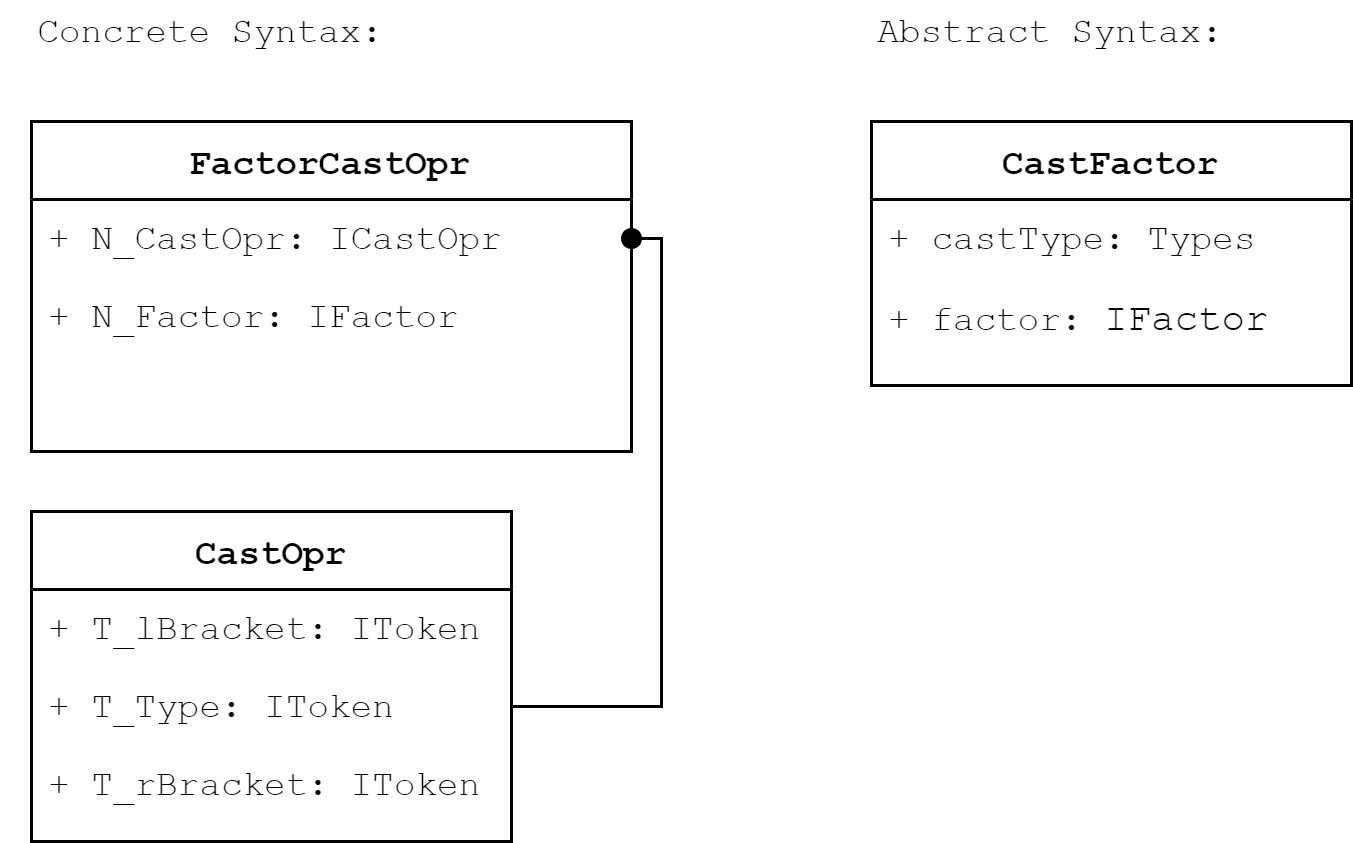
\includegraphics[width=\linewidth]{uml_ast.png} % Figure image
    \caption{Umwandlung von der konkreten in die abstrakte Syntax} % Figure caption
    \label{ast}
\end{figure}
\subsection{Statische Analyse}
% TODO: Beschreiben, dass && und || implementiert wurden

\subsubsection*{Scope checking}
Für Routinen und Variablen liegen unterschiedliche Namespaces vor.
Namen für Routinen und Variabeln können deshalb identisch sein.
Es wird zwischen globalen und lokalen Namespaces unterschieden: Bei lokalen Namespaces werden die Variable innerhalb einer Routine definiert und haben dort ihre Gültigkeit.
Globale Variabeln dürfen nicht denselben Namen haben wie lokalen Variabeln.
Überladene Signaturen für Routinen\footnote{selber Name, unterschiedliche Parameterlisten} wurde in dieser Implementation nicht umgesetzt.

Bei \textit{FunCallFactor, ProcCallCmd, DebugIn} und \textit{AssignCmd} muss überprüft werden, ob die Parameter den richtigen \texttt{LValue}, resp. \texttt{RValue} besitzen.
Folgende Kombinationen sind dabei allgemein erlaubt:

\begin{table}[h]
    \centering
    \tiny
    \caption{LRValue-Kombinationen}
    \label{tab:lrvalues}
    \resizebox{\columnwidth}{!}{%
    \begin{tabular}{@{}lll@{}}
        \toprule
        Callee & Caller & Resultat                       \\ \midrule
        LValue & LValue & Valid                          \\
        RValue & LValue & Valid (LValue dereferenzieren) \\
        RValue & RValue & Valid                          \\
        LValue & RValue & LRValueError \Lightning         \\ \bottomrule
    \end{tabular}%
    }
\end{table}
Bei einem \textit{AssignCmd} muss der Ausdruck links zudem zwingend ein \texttt{LValue} sein.
Bei einem \textit{DebugIn} muss es sich ebenfalls um einen \texttt{LValue} handeln, damit der Input-Wert dieser Variable zugewiesen werden kann.

Innerhalb des Scope checkings wird zudem überprüft, ob die Anzahl der erwarteten Parameter mit der Anzahl übergebener Parameter übereinstimmt.

\subsubsection*{Type checking}
Das Casten zwischen zwei Datentypen ist nur für bestimmte Typen erlaubt (vgl. Tabelle \ref{tab:Casting}).
Zusätzlich sind bei der Abarbeitung des AST nur die folgenden Typen erlaubt:

\begin{table}[h]
    \centering
    \tiny
    \caption{Erlaubte Typen}
    \label{tab:types}
    \resizebox{\columnwidth}{!}{%
    \begin{tabular}{@{}ll@{}}
        \toprule
        Klasse & Types \\ \midrule
        AddExpr, MultExpr, RelExpr      & \texttt{int64, nat64} * \\
        BoolExpr, IfCmd                 & \texttt{bool} \\
        AssignCmd                       & \texttt{int64, nat64, bool} * \\
        FunCallFactor, ProcCallFactor   & Typ von Caller muss \\
                                        & Typ von Callee entsprechen \\
        MonadicFactor                   & NOTOPR: \texttt{bool} \\
                                        & ADDOPR: \texttt{int64, nat64} \\
        CastFactor                      & Typ von Factor und \\
                                        & Typ von CastFactor \\
                                        & müssen castable sein\\ \bottomrule
    \end{tabular}%
    }
\end{table}
Bei Einträgen, die mit * gekennzeichnet sind, müssen \texttt{LValue} und \texttt{RValue} vom selben Typ sein.
Beim der Typenüberprüfung innerhalb vom \texttt{CastFactor} wird überprüft, ob der Typ vom \texttt{CastFactor} und jener des zugehörigen \texttt{factors} gecasted werden können (vgl. Tabelle \ref{tab:Casting}).
Die effektive Typ-Konversion wird erst bei der Code-Generierung durchgeführt.

\subsubsection*{Initalization checking}
% TODO: Beschreiben anhand von Methode doInitChecking und Code in den ensprechenden Klassen refactoren und Variabeln umbenennen etc.

\subsection{Virtuelle Maschine}
Grundlage für die Code-Generierung ist der Abstract Syntax Tree (AST).
Vom Root-Knoten ausgehend fügt jeder Knoten seinen Code zum Code-Array.

Im Falle eines Castings zwischen zwei Datentypen befindet sich an mindestens einer Stelle in der AST Struktur ein \texttt{CastFactor}-Element.
% TODO: Irgendwo vorher beschreiben, dass castOpr in cst zu CastFactor in ast wird
Von diesem Element aus wird der Datentyp des zugehörigen \texttt{factor} geändert, indem dessen Attribut \texttt{castFactor} geändert wird.
Dieses Attribut übersteuert den eigentlichen Datentyp des Elements innerhalb des AST.
Weil der \texttt{factor} gemäss Grammatik unterschiedliche Produktionen besitzt (vgl. Änderungen an der Grammatik), muss die Typanpassung rekursiv weitergegeben werden.
Die Rekursion wird durch Literale oder Expressions unterbrochen, wie am Beispiel in Anhang \ref{bsp_casting} aufgezeigt.

In der virtuellen Maschine wurde ein neuer generischer Typ \texttt{NumData} eingeführt.
Dieser wird für die Konversion zwischen Daten vom Typ \texttt{IntData}\footnote{für den Datentyp \texttt{int64}} und \texttt{NatData}\footnote{für den Datentyp \texttt{nat64}} verwendet.
Abbildung \ref{data_hierarchy} zeigt die Klassenhierarchie dieser Typen.

\begin{figure}[H]
    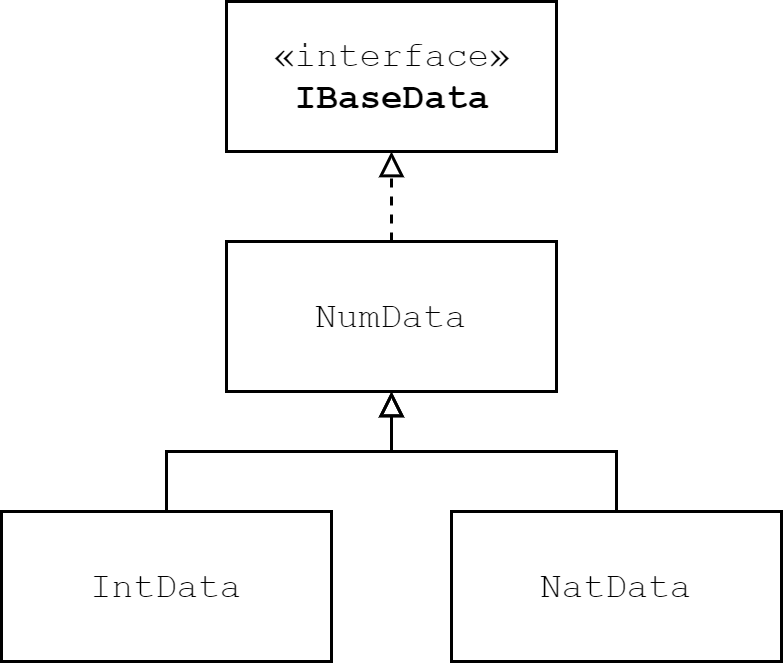
\includegraphics[width=\linewidth]{uml_data_hierarchy.png} % Figure image
    \caption{Daten in VM} % Figure caption
    \label{data_hierarchy}
\end{figure}

\subsection{Code Generierung}
% TODO Eigentlich kein separates Kapitel

\section{Vergleich mit anderen Programmiersprachen}
\subsection{Ganzzahlige Werte}
In Java wird bei Zuweisungen die Länge einer Zahl in Bitdarstellung überprüft:
Beim Datentyp \texttt{long} wird beispielsweise geprüft, ob der Wert als ganzzahliger Wert von 64-bit Länge dargestellt werden kann.
Falls dies nicht der Fall ist, wird ein Fehler zur Kompilierungszeit geworfen.
Das MSB wird als Vorzeichenbit verwendet, womit rund die Hälfte der vorzeichenlos darstellbaren \texttt{long}-Werte entfällt, resp. zur Darstellung von negativen Zahlen eingesetzt wird.
Falls bei fortlaufenden Berechnungen Wertebereiche unter- resp. überschritten werden, führt dies zu einem arithmetischen Überlauf.
Abbildung \ref{zahlenkreis} %TODO: Abbildung-Nr.verifizieren
zeigt den Überlauf bei ganzzahligen, vorzeichenbehafteten Datentypen (am Beispiel von Bitlänge 3 + 1).

\begin{figure}[H]
    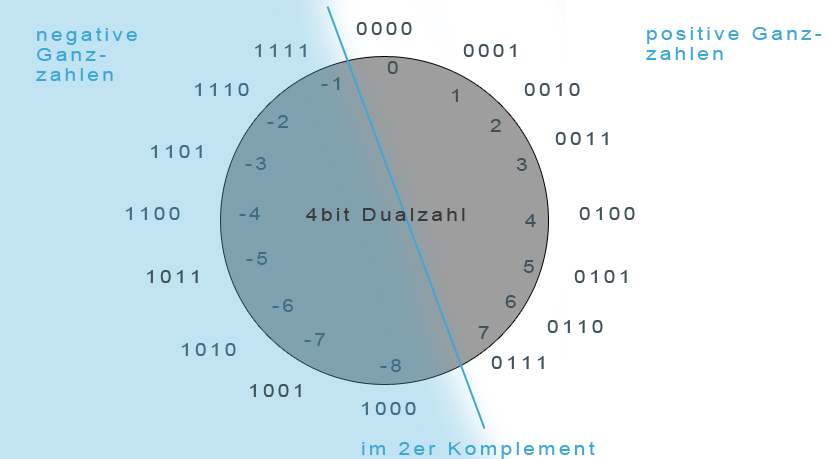
\includegraphics[width=\linewidth]{zahlenkreis_int3.jpg} % Figure image
    \caption{Überlauf mit Integerzahlen } % Figure caption
    % TODO: Ref: https://de.wikipedia.org/wiki/Integer_(Datentyp)#/media/Datei:Zahlenkreis_sint3.jpg
    \label{zahlenkreis}
\end{figure}


Dadurch führt z.B. beim Datentyp \texttt{int} der Ausdruck \texttt{Integer.MAX\_VALUE + 1} zum Wert \texttt{Integer.MIN\_VALUE}.
Dies kann dazu führen, dass mit \glqq falschen\grqq \ Werten gerechnet wird, ohne dass der Entwickler dies bemerkt.

\subsection{Fliesskommazahlen}
% TODO: Zweierkomplement oben noch nicht beschrieben
Im Gegensatz zur Darstellung im Zweierkomplement, welche für Integer-Typen in Java verwendet werden, werden Fliesskommazahlen intern nach IEEE Standard dargestellt.
Anders als bei der Zweierkomplement-Darstellung sieht dieses Format spezielle, konstante Werte vor.
So sind in Java beispielsweise Konstanten für \texttt{Double.POSITIVE\_INFINITY}, \texttt{Double.NEGATIVE\_INFINITY} und \texttt{Double.NaN} definiert.
%  Quelle: https://stackoverflow.com/questions/41312477/purpose-of-defining-positive-infinity-negative-infinity-nan-constants-only-for

\section{Designentscheidungen}
\subsection{Spezifiziertes Verhalten}
Der neue Datentyp \texttt{nat64} unterstützt die bestehenden Operationen aus IML\footnote{Aktuell sind dies \begin{itemize}
                                                                                                                \item MULTOPR(*, divE, modE) \item ADDOPR(+, -) \item RELOPR(<, <=, >, >=, =, /=) \item BOOLOPR(&&, ||, &, |)
\end{itemize}}.
Sofern sich die einzelnen Operanden und auch das Resulat im Wertebereich\footnote{$[0,4294967295]$} befinden,
entspricht das Verhalten vom Datentyp \texttt{nat64} jenem vom Datentyp \texttt{int64}.
Andernfalls wird folgendes Verhalten festgelegt:

\begin{itemize}
    \item \textbf{Wertebereich}: Wertebereichsüber- resp. Unterschreitungen resultieren in einem Laufzeitfehler\footnote{Negative Zahlen entsprechen Wertebereichsunterschreitungen}. Dies erhöht die Typsicherheit beim Einsatz der verschiedenen Datentypen.
    \item \textbf{Nachkommastellen}: Gemäss IML-Spezifikation sind als Literale nur ganzzahlige Werte erlaubt. Falls z.B. bei einer Division ein Rest resultiert, wird ein ganzzahliges Resultat zurückgegeben. Der Wert des Resultats ist abhängig von der gewählten Operation (\texttt{DivFloor, \texttt{DivTrunc}, etc.).}
\end{itemize}

\subsection{Alternative Ansätze}
% TODO: Alternativen beschreiben
% a) Arithmetischer Überlauf ohne Anzeigen, Doppelt soviele Werte wie int
% c) Inf. wie bei Double
% d) Unser Ansatz (negative Werte als Abosulte Werte, bei Überschreitungen mit max weiterrechnen)
% TODO: Downsides z.B. gemäss %  Quelle: https://stackoverflow.com/questions/41312477/purpose-of-defining-positive-infinity-negative-infinity-nan-constants-only-for

\section{Beispielprogramme}
\label{sec:prog}
Operation:
\begin{lstlisting}
    program progAddition
    global
    var x:nat64;
    var y:nat64;
    var r:nat64;
    var b:bool
    do
    x init := 4;
    y init := 3;
    r init := x + y;
    b init := r = 7;

    debugout r;
    debugout b
    endprogram
\end{lstlisting}
Casting:
\begin{lstlisting}
    program progCasting
    global
    var x:nat64;
    var y:int64;
    var r:nat64;
    var b:bool
    do
    x init := 4;
    y init := 3;
    r init := x + [nat64] y;
    b init := r = 7;

    debugout r;
    debugout b
    endprogram
\end{lstlisting}

%----------------------------------------------------------------------------------------
%	BIBLIOGRAPHY
%----------------------------------------------------------------------------------------

\begin{thebibliography}{9}
    \bibitem{wikipedia}
    Wikipedia: Natürliche Zahl,
    \url{https://de.wikipedia.org/wiki/Nat\%C3\%BCrliche_Zahl}

    \bibitem{wikipedia}
    Wikipedia: Natural numbers (engl.),
    \url{https://en.wikipedia.org/wiki/Natural_number}
\end{thebibliography}

%----------------------------------------------------------------------------------------
%	APPENDIX
%----------------------------------------------------------------------------------------
\clearpage
\appendix
\section{Vollständige Grammatik}
% TODO

\clearpage
\section{Beispiel doppeltes Casting}
\label{bsp_casting}
IML:
\begin{lstlisting}
    program progDouble
    global
    var value:int64
    do
    value init := [int64] [nat64] ((4 + 1) + 1)
    endprogram
\end{lstlisting}

Code-Array:
\begin{lstlisting}
    0: AllocBlock(1)
    1: UncondJump(2)
    2: LoadAddrAbs(0)
    3: LoadImInt(4)
    4: LoadImInt(1)
    5: AddInt
    6: LoadImInt(1)
    7: AddInt
    8: Store
    9: Stop
\end{lstlisting}

UML:
\begin{figure}[H]
    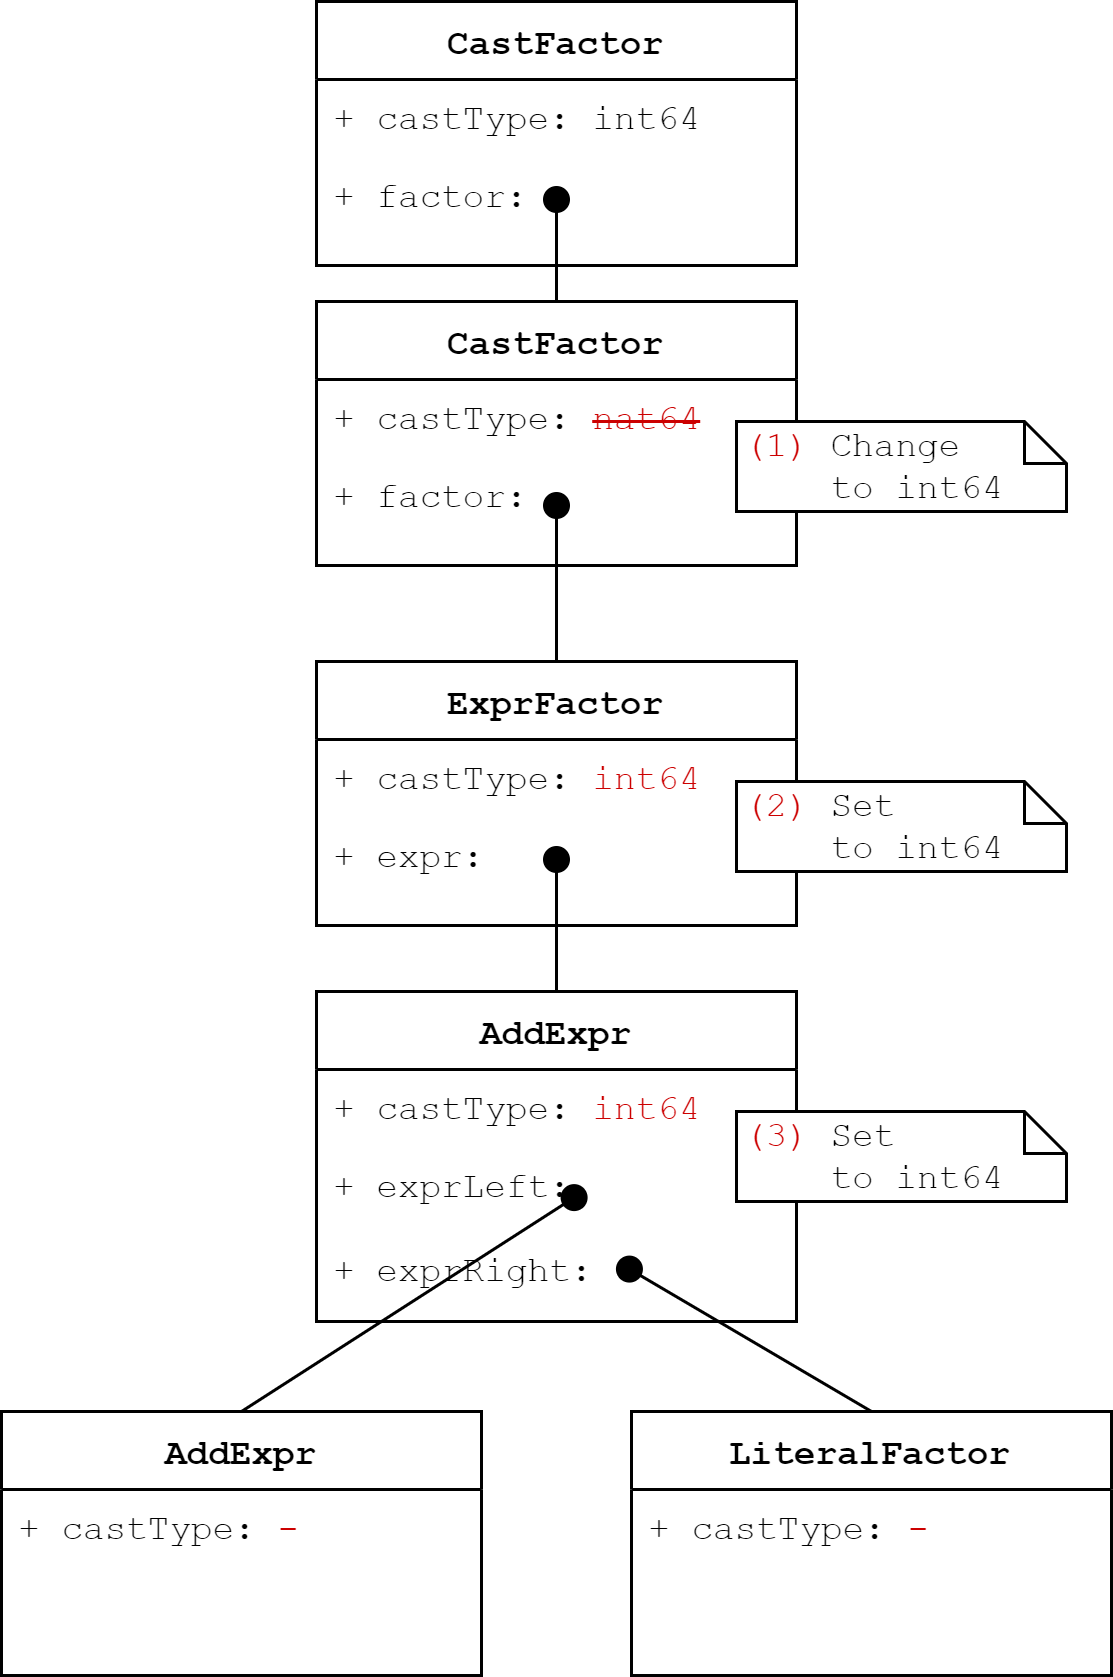
\includegraphics[width=\linewidth]{uml_casting.png} % Figure image
    \caption{Auszug aus AST } % Figure caption
    \label{casting}
\end{figure}


%----------------------------------------------------------------------------------------

\end{document}
